\vspace{-1mm}
\section{Experimental Evaluation}
\label{sec:experiments}
\vspace{-1mm}

In this Section, we investigate what effect \agentsmds{} have on the behavior of coding agents and how strong this effect is. To this end, we conduct an extensive evaluation of various coding agents on \swebench{} and \planbench{}, considering both automatically generated and developer-provided \agentsmds{}.

\begin{figure*}[t]
    \centering
    \hspace*{\fill}
    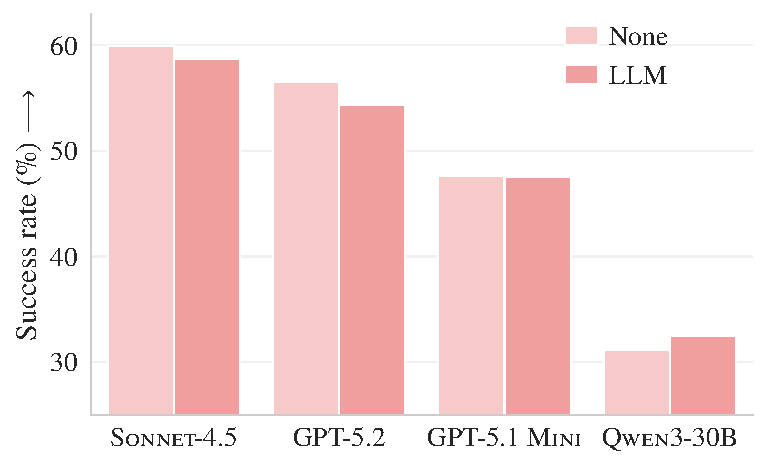
\includegraphics[width=.42\linewidth]{figures/main_eval/perf/experiment1_accuracy_swebench.pdf}
    \hspace*{\fill}
    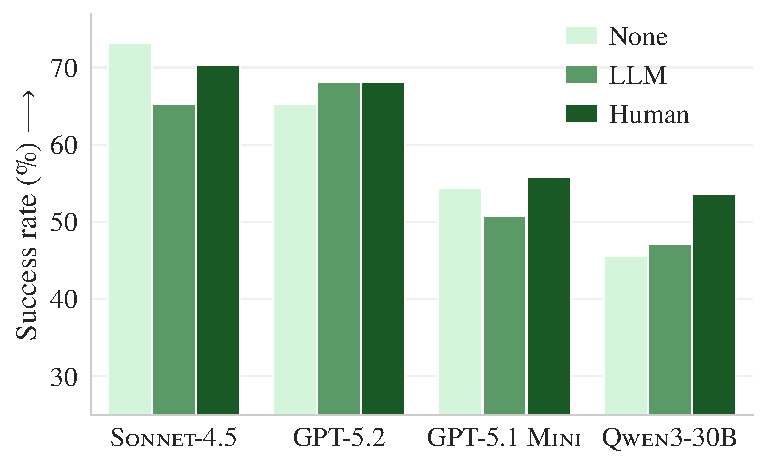
\includegraphics[width=.42\linewidth]{figures/main_eval/perf/experiment1_accuracy_planbench.pdf}
    \hspace*{\fill}
    \caption{Resolution rate for 4 different models, without \agentsmds{}, with LLM-generated \agentsmds{}, and with developer-written \agentsmds{}, on \colorbox{swebenchcolor}{\swebench{}} (left) and \colorbox{planbenchcolor}{\planbench{}} (right).
    }
    \label{fig:exepriment1_perf}
\end{figure*}

\subsection{Experimental Setup}

We describe the experimental setup below, deferring further details to \cref{app:experiments:setup}.


\paragraph{Coding Agents}
We consider four coding agents, paired with suitable models: \claudecode{} \citep{ClaudeCodeDocsOverview} with \sonnet{}~\citep{sonnet45}, \codex{} \citep{openaiCodex2026} with \gptfive{} and \gptfivemini{} \citep{singh2025openaigpt5card}, and \qwencode{} \citep{QwenLMQwen3Coder} with \qwen{}~\citep{qwen3}.
For \claudecode{}, we use the default settings and set the temperature of \sonnet{} to $0$.
Similarly, for \codex{}, we also use the default settings and set the temperature of \gptfive{} and \gptfivemini{} to $0$.
For \qwencode{}, we enable chat compression upon reaching $60$\% of the total context limit (set to $256$K tokens), restrict shell outputs to $2000$ tokens, and set the temperature of \qwen{} to $0.7$ with top-$p$ sampling at $0.8$. We deploy \qwen{} locally using vLLM~\citep{vllm}. We sample completions for each agent once.
For all agents, the \agentsmd{} is fed into their context, either by writing it to \texttt{AGENTS.md} for \codex{} and \qwencode{}, or to \texttt{CLAUDE.md} for \claudecode{}.

\paragraph{Datasets}
We use \swebench{} \citep{swebench}, which consists of 300 tasks sourced from GitHub issues across 11 popular Python repositories, none containing developer-written \agentsmds{}, and our novel \planbench{}, consisting of 138 instances from 12 repositories, all containing developer-provided \agentsmds{} (see \cref{sec:method}).

\paragraph{Settings}
We consider three \agentsmd{} settings:
\begin{enumerate}
    \vspace{-2mm}
    \item[]\hspace{-2mm}\noplan{}: No \agentsmds{} are available, i.e., we remove developer-provided files for \planbench{}.
    \item[]\hspace{-2mm}\autoplan{}: An LLM-generated \agentsmd{} is available. We use the recommended initialization command and model for each agent individually to generate the \agentsmd{} using the pre-patch repository state $R$.
    \item[]\hspace{-2mm}\humanplan{}: A developer-provided \agentsmd{} is available. We use the \agentsmd{} of the pre-patch repository state $R$. Only available for \planbench{}.
\end{enumerate}

\paragraph{Metrics}
The main metric for agent performance is success rate (\cref{sec:notation-success}), i.e., the portion of instances for which the agent produces a patch that leads to all tests passing. 
We additionally consider the number of \emph{steps} the agent requires to complete a task. 
Each step is one interaction with the environment, e.g., calling a shell tool or modifying a file. 
Finally, we report the total \emph{cost} of LLM inference required to complete a task.
For \qwen{}, we estimate the cost from the average OpenRouter API price.

\subsection{Main Results}
\label{sec:eval:main}

\begin{figure*}[t]
    \centering
    \hspace*{\fill}
    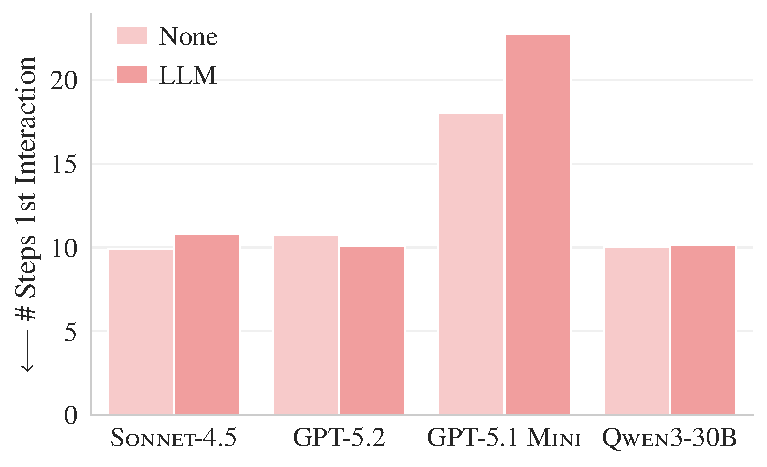
\includegraphics[width=.42\linewidth]{figures/main_eval/interaction_speed/experiment1_stepsfirstread_swebench.pdf}
    \hspace*{\fill}
    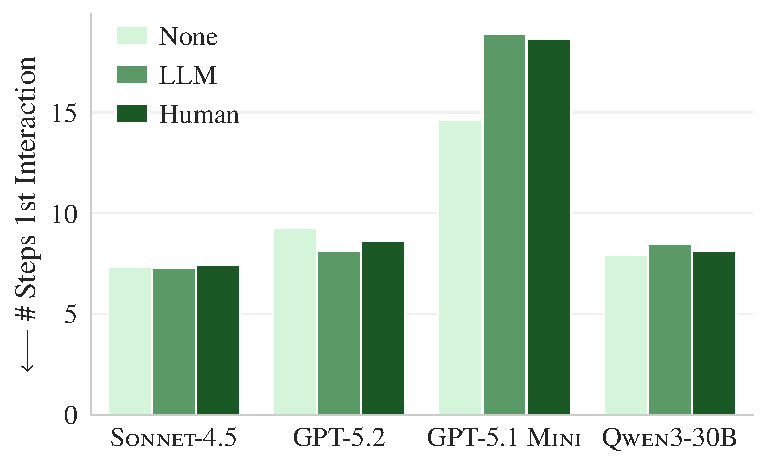
\includegraphics[width=.42\linewidth]{figures/main_eval/interaction_speed/experiment1_stepsfirstread_planbench.pdf}
    \hspace*{\fill}
    \caption{Number of steps before the first interaction between the agent and a file included in the PR patch (lower is better) is generally lower without \agentsmds{} than with LLM-generated \agentsmds{} or with developer-written \agentsmds{} (Human) on \colorbox{swebenchcolor}{\swebench{}} (left) and \colorbox{planbenchcolor}{\planbench{}} (right).
    }
    \label{fig:exepriment1_speed}
\end{figure*}


\begin{table}[t]
\caption{The average number of steps (lower is better) and execution cost (in USD --- lower is better) per \swebench{} and \planbench{} instance without \agentsmds{} (\noplan), with LLM-generated \agentsmds{} (LLM), and with developer-written \agentsmds{} (\textsc{Hum}). We \textbf{bold} the best setting.}
\label{tab:main_cost}
\centering
\resizebox{\linewidth}{!}{
\begin{tabular}{ll cc cc cc cc}
\toprule
& \multirow{2}{*}{Type} & \multicolumn{2}{c}{\sonnet{}} & \multicolumn{2}{c}{\gptfive{}} & \multicolumn{2}{c}{\textsc{GPT-5.1 M.}} & \multicolumn{2}{c}{\textsc{Qwen3-30B}} \\
\cmidrule{3-10}
&& Steps & Cost & Steps & Cost & Steps & Cost & Steps & Cost \\
\midrule
\multirow[c]{2}{*}{\shortstack[c]{\textsc{SWE-}\\\textsc{Bench}\\\textsc{Lite}}} & \noplan{} & \textbf{54.4} & \textbf{1.30} & \textbf{12.5} & \textbf{0.32} & \textbf{40.9} & \textbf{0.18} & \textbf{29.7} & \textbf{0.12} \\
\cmidrule{2-10}
& LLM & 57.2 & 1.51 & 12.7 & 0.43 & 45.2 & 0.22 & 32.2 & 0.13 \\
\midrule
\multirow[c]{4}{*}{\shortstack[c]{\textsc{Agent-}\\\textsc{bench}}} & \noplan & \textbf{40.7} & \textbf{1.15} & \textbf{12.1} & \textbf{0.38} & \textbf{40.6} & \textbf{0.18} & \textbf{31.5} & \textbf{0.13} \\
\cmidrule{2-10}
& LLM & 46.5 & 1.33 & 13.1 & 0.57 & 46.9 & 0.20 & 34.2 & 0.15 \\
\cmidrule{2-10}
& \textsc{Hum.} & 45.3 & 1.30 & 13.6 & 0.54 & 46.6 & 0.19 & 32.8 & 0.15 \\
\bottomrule 
\end{tabular}}
\end{table}


\paragraph{LLM-generated \agentsmds{} increase cost and reduce performance}
LLM-generated \agentsmds{} cause performance drops in 5 out of 8 settings across \swebench{} and \planbench{} (see \cref{fig:exepriment1_perf}).
In more detail, the average resolution rate is reduced by $0.5\%$ and $2\%$ on average on \swebench{} and \planbench{}, respectively.
Meanwhile, the \agentsmds{} increase the \# steps in every setting on average by $2.45$ and $3.92$ steps, respectively, which leads to a cost increase of 20\% and 23\% on average, respectively (see \cref{tab:main_cost}).


\paragraph{Human \agentsmds{} increase cost and performance}
We observe that the developer-provided \agentsmds{} outperform the LLM-generated ones for all four agents, despite not being agent-specific, and improve the performance compared to no \agentsmds{} for all agents but \claudecode{} (see \cref{fig:exepriment1_perf} right).
However, developer-provided \agentsmds{} also increase the average number of steps and costs required to solve the task, on average by $3.34$ steps and at most 19\%, respectively.

\paragraph{\Agentsmds{} do not provide effective overviews}
One recommendation for \agentsmds{} is to include a codebase overview~\citep{AGENTSMd2025}.
Across the 12 developer-provided \agentsmds{} in \planbench{}, 8 include a dedicated codebase overview, with 4 explicitly enumerating and describing the directories and subdirectories in the repository.
Similarly, both the \codex{} and \qwencode{} \agentsmd{} generation prompts explicitly instruct the agent to include an overview section, while the \claudecode{} prompt advocates for a high-level overview only and warns against listing components that are easily discoverable.
We use \gptoss{} to assess which of the LLM-generated \agentsmds{} contain codebase overviews.
Surprisingly, $100\%$ of \sonnet{}-generated \agentsmds{} are flagged for overviews, and $95\%$ and $99\%$ for \qwen{} and \gptfive{} respectively. Only \gptfivemini{} has significantly fewer overviews ($36\%$).

\begin{figure}[t]
    \centering
    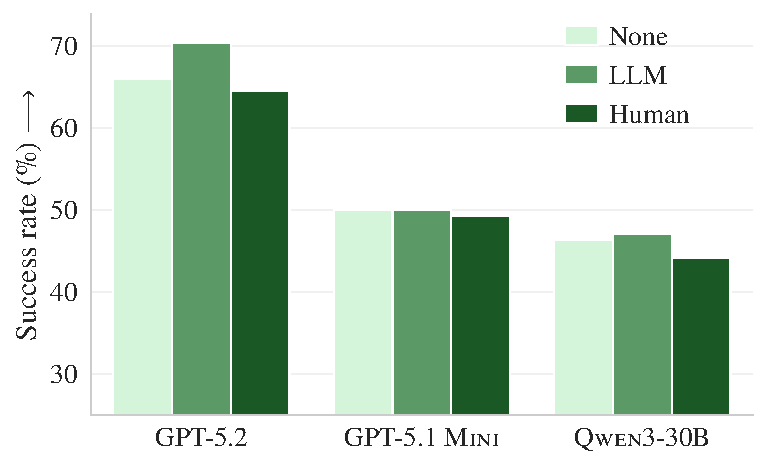
\includegraphics[width=.8\linewidth]{figures/main_eval/nodocs/experiment4_accuracy_planbench.pdf}
    \caption{When removing all documentation-related files from the codebase, LLM-generated \agentsmds{} tend to outperform developer-provided (Human) ones on \colorbox{planbenchcolor}{\planbench{}}.
    }
    \label{fig:experiment4_perf}
\end{figure}

\begin{figure*}[t]
    \centering
    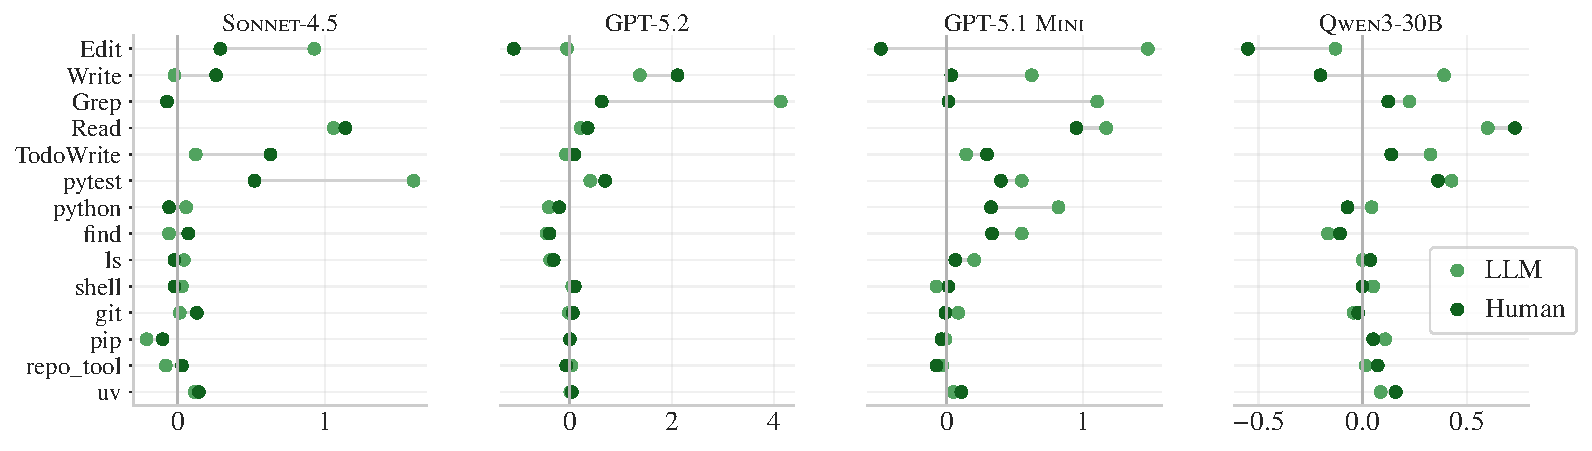
\includegraphics[width=\linewidth]{figures/main_eval/tool_freq/experiment1_tool_freq_pdf.pdf}
    \caption{Increase in average tool use when including LLM-generated (bright green) or developer-provided (dark green) \agentsmds{}, compared to the average tool use without \agentsmds{}. For tool names, we map \codex{} and \qwencode{} tools to the \claudecode{} equivalents (we detail the mapping in \cref{app:experiments}).}
    \label{fig:experiment1_tool_freq}
\end{figure*}


To assess the usefulness of these overviews, we measure how quickly agents discover files relevant to the described issue $I$.
Concretely, we measure the average number of steps before the coding agent interacts with any file modified in the original PR patch $X^{*}$.
We exclude the $3\%$ of instances in which the agent never interacts with any file modified in $X^{*}$. 
Both on \swebench{} and \planbench{} the presence of \agentsmds{} does not meaningfully reduce this metric, as shown in \cref{fig:exepriment1_speed}.

While \agentsmds{} appear to increase the number of required steps significantly for \gptfivemini{}, we observe in manual trace inspection that this increase is due to it (i) issuing multiple commands to find the \agentsmds{} and (ii) reading them (multiple times) despite them being already included in the agent's context. Interestingly, we only observed this behavior if \agentsmds{} were present at all.
We conclude that \agentsmds{}, even developer-provided ones, are not effective at providing a repository overview.


\paragraph{\Agentsmds{} are redundant documentation}
Our hypothesis is that LLM-generated \agentsmds{} are highly redundant with existing documentation, while developer-provided \agentsmds{} add additional information.
To confirm this, we manually remove all documentation (files ending with \texttt{.md}, example code, and the folder \texttt{docs/}) after generating the \agentsmd{}, and before evaluating the coding agents. We show the results in \cref{fig:experiment4_perf}, excluding \claudecode{} due to its hight cost.
In this setting, where \agentsmds{} are the only source of documentation available, LLM-generated \agentsmds{} not only consistently improve performance by $2.7$\% on average, but also outperform developer-written documentation.
This may explain anecdotal evidence reporting that coding agents perform better after adding \agentsmds{}~\citep{builderioImproveYourAICodeOutputWithAgentsMd}, since many less popular repositories contain little to no documentation.


\subsection{Trace analysis}
\label{sec:eval:trace}

We now analyze the impact of \agentsmds{} on agent behavior in more detail by analysing the frequency of agent tool calls and length of reasoning traces. We describe our setup in more detail in \cref{app:prompts:trace_analysis}.


\paragraph{\Agentsmds{} lead to more testing and exploration}
In \cref{fig:experiment1_tool_freq}, we show the increase in average tool use when including LLM-generated (bright green) or developer-provided (dark green) \agentsmds{}. Negative values imply a decrease in tool use. We find that, across all models, when \agentsmds{} are present, the coding agents run more tests.
They also tend to navigate the repository more: they search more files (\texttt{grep}), read more files, and write more files.
Lastly, adding \agentsmds{} causes agents to use more repository-specific tooling (\eg \texttt{uv} and \texttt{repo\_tool}).
In \cref{fig:experiment1_toolintent_freq} (\cref{app:experiments}), we perform a similar analysis using the intent of the tool call, leading to the same conclusion.

\paragraph{Instructions in \agentsmds{} are typically followed}
We find that agents generally follow instructions present in the \agentsmds{}.
For instance, \texttt{uv} is used 1.6 times per instance on average when mentioned in the \agentsmds{}, compared to fewer than 0.01 times when it is not mentioned, and repository-specific tools are used 2.5 times per instance on average when mentioned, compared to fewer than 0.05 times when they are not mentioned.
This effect is observable across almost all measured tools displayed in \cref{fig:experiment1_tool_freq}, as we show in a more in-depth analysis in \cref{app:experiments}.
In particular, this result implies that the absence of improvements with \agentsmds{} is not due to a lack of instruction-following.

\begin{figure}[t]
    \centering
    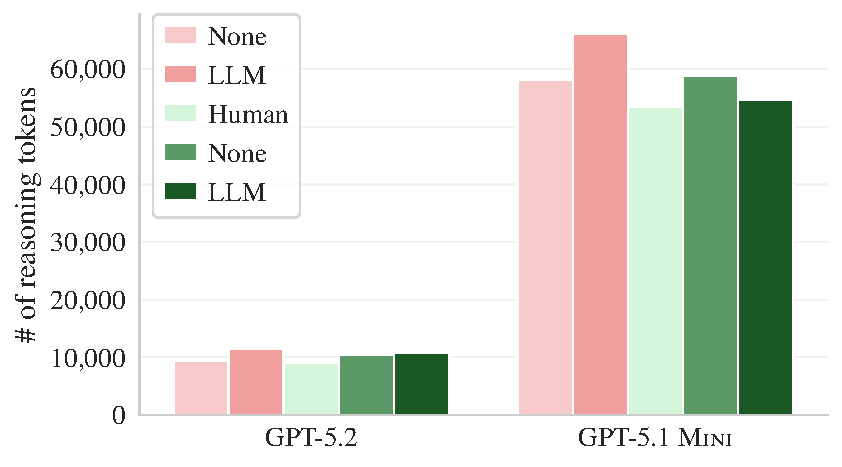
\includegraphics[width=\linewidth]{figures/main_eval/ttc/experiment1_ttc_both.pdf}
    \caption{Number of reasoning tokens spent on average by \gptfive{} and \gptfivemini{}, without \agentsmds{}, with LLM-generated \agentsmds{}, and with developer-written \agentsmds{}, on \colorbox{swebenchcolor}{\swebench{}} (left) and \colorbox{planbenchcolor}{\planbench{}} (right).}
    \label{fig:exepriment1_ttc}
\end{figure}


\paragraph{Following \agentsmds{} requires more thinking}
We hypothesize that these additional instructions make the task harder.
To confirm this, we analyze the average number of reasoning tokens used by \gptfive{} and \gptfivemini{}, as their adaptive reasoning~\citep{adaptive_reasoning} allows them to use more reasoning tokens for tasks that they deem harder.
In \cref{fig:exepriment1_ttc}, we show that LLM-generated \agentsmds{} indeed increase the average number of reasoning tokens by 22\% for \gptfive{} and 14\% for \gptfivemini{} on \swebench{} (respectively 14\% and 10\% on \planbench{}), and that developer-written \agentsmds{} increase the number of reasoning tokens by 20\% and 2\% for \gptfive{} and \gptfivemini{}, respectively.


\subsection{Ablations}

In this Section we analyze differences between the \agentsmds{} generated by different models, and the impact of the prompt used to create the \agentsmds{}.

\begin{figure}[t]
    \centering
    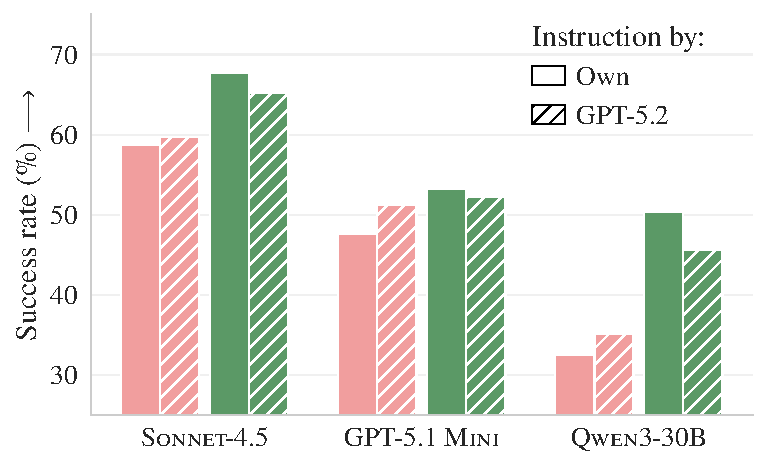
\includegraphics[width=.85\linewidth]{figures/ablation_big_plan/experiment2_accuracy.pdf}
    \caption{On \colorbox{swebenchcolor}{\swebench{}}, performance is improved with \agentsmds{} generated by \gptfive{} compared to using the model underlying the agent, while on \colorbox{planbenchcolor}{\planbench{}} performance is degraded.
    }
    \label{fig:experiment2_perf}
\end{figure}


\paragraph{Stronger models don't generate better \agentsmds{}}
We compare \agentsmds{} generated with \gptfive{} + \codex{} to those created by our standard agents in \cref{fig:experiment2_perf}.
This improves performance on \swebench{} across all models (2\% on average), but degrades performance on \planbench{} across all models (3\% on average).
We thus conclude that stronger models do not necessarily generate superior \agentsmds{}.

\begin{figure}[t]
    \centering
    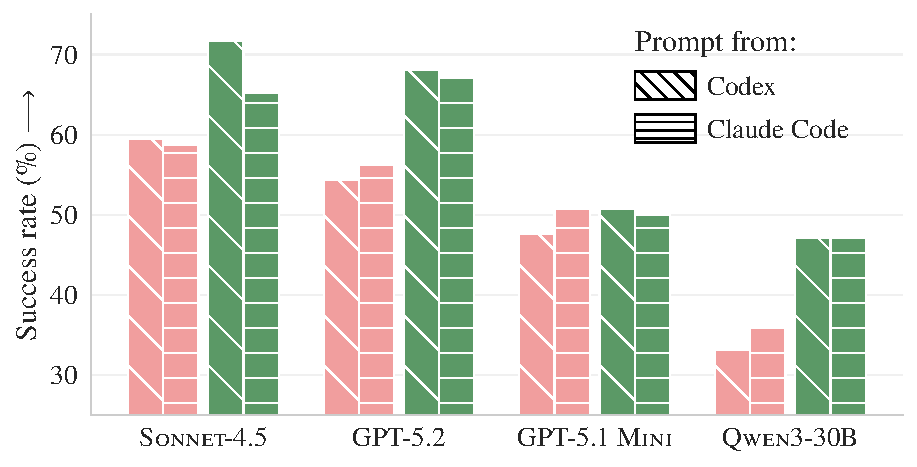
\includegraphics[width=\linewidth]{figures/ablation_prompt/experiment3_accuracy.pdf}
    \caption{When generating \agentsmds{} using the prompt from \codex{} or from \claudecode{} on \colorbox{swebenchcolor}{\swebench{}} and \colorbox{planbenchcolor}{\planbench{}}, there is no consistent impact on success rate.
    }
    \label{fig:experiment3_perf}
\end{figure}


\paragraph{No difference between the specific prompts}
We compare \agentsmds{} generated using the prompt of \codex{} and \claudecode{} across all agents and models in \cref{fig:experiment3_perf}.
Surprisingly, \claudecode{} performs better with \agentsmds{} generated using the \codex{} prompt, while both \gptfive{} and \gptfivemini{} perform better on \swebench{} with the \codex{} prompt but worse on \planbench{}.
Overall, neither the prompt matching the underlying model and agent, nor a specific prompt performs consistently best, indicating that sensitivity to different (good) prompts is generally small.
